\chapter{界面处的反射与透射}\label{ch:b2:wave-interfaces}

超声医师在探头与皮肤之间挤入耦合凝胶：
没有它，声波会被薄薄的空气层反射回去，永远无法进入
人体。照相机镜头镀有一层四分之一波长厚的膜，
其表面便不再反射。无线电波遇到电离层便折返；
光遇到银镜也会折返；
脉冲到达电缆末端后，以倒相或同相返回，
具体取决于末端所接的负载。每一种波遇到介质变化时，
都会分为反射与透射两部分，并由一个思想
决定两部分的比例：界面处的\emph{连续性条件}，
它用两种介质的阻抗来表示。本章将其应用于
声波、两种\omterm{prop:b2:waves-in-media:lorentz}{电介质}之间的光、\omterm{def:b2:waves-in-media:plasma}{等离子体}、金属，
以及电缆，并由此导出反射定律与折射定律，
还有玻璃恰好不反射的那个角度。

\begin{omfigure}
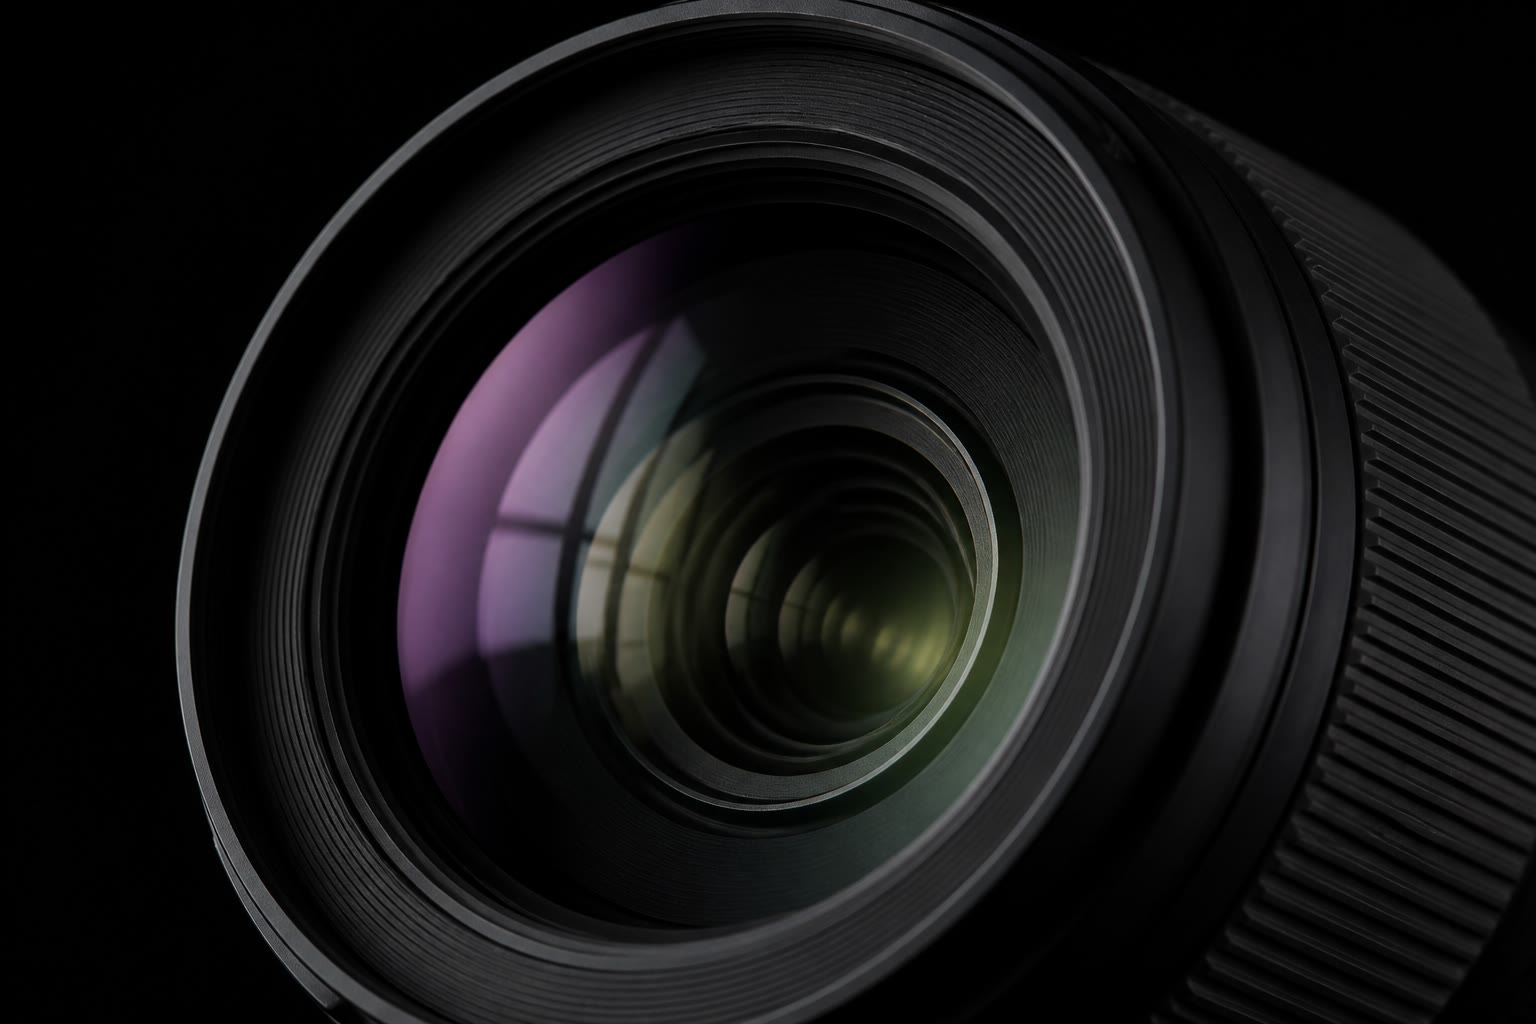
\includegraphics[width=0.54\linewidth]{images/book4/ai/b4-15-coated-camera-lens.jpg}

{\small 多层镀膜的照相机镜头：淡紫色与绿色的反光，是每个裸玻璃表面本应反射的 4\% 中残余的部分。}
\end{omfigure}


\section{垂直入射：阻抗规则}

\begin{theorem}[垂直入射时的反射与透射]\label{thm:b2:wave-interfaces:normal}
\index{反射系数}\index{透射系数}\index{阻抗匹配}
平面波在介质 1 中射向位于 $x = 0$ 处的平面界面，该界面另一侧为
介质 2。每种介质由阻抗 $Z_i$ 表征（阻抗是界面处两个连续场量之比
——对声波为压强与
速度，对光为 $E$ 与 $H = B/\mu_0$，对\omterm{prop:b2:dispersion-wave-packets:coax}{传输线}为电压与
电流）。两个量在 $x = 0$ 处都连续，由此对
“力类”量（压强、$E$、$v$）有
\[
r = \frac{Z_2 - Z_1}{Z_2 + Z_1} , \qquad t = \frac{2Z_2}{Z_2 + Z_1} ,
\qquad R = r^2 , \quad T = \frac{4Z_1Z_2}{(Z_1 + Z_2)^2} , \quad R + T = 1 .
\]
（对于“流类”量——速度、$H$、电流——$r$
符号改变。）当 $Z_1 = Z_2$ 时无任何反射（\emph{匹配}介质）；
当 $Z_2 \gg Z_1$（$r \to +1$）或 $Z_2 \ll Z_1$（$r \to -1$）时，几乎全部被反射。
\end{theorem}

\begin{proof}
入射波 $p_i = A\cos(\omega t - k_1x)$，反射波 $p_r = rA\cos(\omega t + k_1x)$，
透射波 $p_t = tA\cos(\omega t - k_2x)$，频率相同。相应的
流量分别为 $p/Z_1$、$-p_r/Z_1$（沿反方向传播的波携带
$v = -p/Z$）以及 $p_t/Z_2$。由 $x = 0$ 处的连续性，有 $1 + r = t$ 与 $(1 - r)/Z_1
= t/Z_2$；解之即得。能量方面，强度为 $p^2/Z$，因此 $R = r^2$ 且
$T = t^2Z_1/Z_2$。
\end{proof}

\begin{example}[三个界面处的声波]\label{ex:b2:wave-interfaces:sound}
空气（$Z = \qty{410}{kg.m^{-2}.s^{-1}}$）到水（$1.5 \times 10^6$）：$r = 0.9995$，
$T = 1.1 \times 10^{-3}$——$99.9\%$ 被反射；游泳者几乎听不到
水面以上世界的动静，超声探头因此需要耦合凝胶。组织
（$1.6 \times 10^6$）到骨（$7 \times 10^6$）：$r = 0.63$，$T = 0.6$。脂肪（$1.38 \times
10^6$）到肌肉（$1.70 \times 10^6$）：$r = 0.10$，$R = 1\%$——图像正是由
这些微弱回波构成的。系在墙上的一根绳（$Z_2 \to \infty$）：对力，$r = +1$；
对速度则为 $-1$，脉冲倒相返回
（见\cref{ch:b2:waves-on-strings}）。
\end{example}

\begin{proposition}[垂直入射时的光；增透膜]\label{prop:b2:wave-interfaces:optics}
\index{反射率（垂直入射）}\index{增透膜}\index{四分之一波长层}
对于折射率分别为 $n_1$、$n_2$ 的两种透明介质间的光（
\omterm{prop:b2:waves-in-media:lorentz}{电介质}的阻抗为 $Z = \sqrt{\mu_0/\varepsilon_0}/n$，与 $n$ 成反比），
对于电场，
\[
r = \frac{n_1 - n_2}{n_1 + n_2} , \qquad R = \Bigl(\frac{n_1 - n_2}{n_1 + n_2}\Bigr)^2 :
\]
每个空气–玻璃界面为 $4\%$，水为 $2\%$，金刚石为 $17\%$。一层
折射率为 $n = \sqrt{n_1n_2}$、厚度为 $\lambda/4n$、置于两介质之间的膜，
使波长 $\lambda$ 处的反射相消（\emph{四分之一波长
\omterm{prop:b2:wave-interfaces:optics}{增透膜}}）：其两表面反射的波振幅相等、
相位相反。同一层若取高折射率，或将交替排列的
\omterm{prop:b2:wave-interfaces:optics}{四分之一波长层}组成叠层，则起相反作用，构成一面
反射率达 $99.99\%$ 的反射镜——即激光器的反射镜。
\end{proposition}

\begin{proof}
切向分量 $\vect E$ 与 $\vect B$ 连续（界面处无\omterm{prop:b2:maxwell-equations:boundary}{面
电流}）：$E_i + E_r = E_t$ 与 $B_i - B_r = B_t$，其中各介质中 $B = nE/c$，
即阻抗规则，$Z \propto 1/n$。对于\omterm{prop:b2:wave-interfaces:optics}{增透膜}，两个反射振幅为
$(n_1 - n)/(n_1 + n)$ 与 $(n - n_2)/(n + n_2)$，
当 $n^2 = n_1n_2$ 时二者相等；光在膜中往返一次所加的相位为
$2\times2\pi n(\lambda/4n)/\lambda = \pi$，因而二者相消（多次反射
影响很小，已包含在\cref{exo:b2:wave-interfaces:5}的精确处理中）。
\end{proof}

\begin{omfigure}
\begin{tikzpicture}[font=\small, x=1cm, y=1cm, >=Stealth]
  \begin{scope}
    \fill[omExo!12] (0,-1.5) rectangle (3.2,1.5); \draw[thick] (0,-1.5) -- (0,1.5);
    \node[font=\footnotesize] at (-1.6,1.25) {$Z_1$}; \node[font=\footnotesize] at (1.6,1.25) {$Z_2$};
    \draw[omDef, very thick, ->] (-3.0,0.5) -- (-0.3,0.5) node[above, pos=0.5, font=\footnotesize] {入射，$1$};
    \draw[omThm, very thick, ->] (-0.3,-0.4) -- (-3.0,-0.4) node[below, pos=0.5, font=\footnotesize] {反射，$r$};
    \draw[omProp, very thick, ->] (0.3,0.2) -- (3.0,0.2) node[above, pos=0.5, font=\footnotesize] {透射，$t$};
    \node[font=\footnotesize] at (0,-2.0) {$r = \dfrac{Z_2 - Z_1}{Z_2 + Z_1}$, $t = \dfrac{2Z_2}{Z_2 + Z_1}$};
  \end{scope}
  \begin{scope}[xshift=8.4cm]
    \fill[omExo!12] (0.8,-1.5) rectangle (3.2,1.5); \fill[omDef!25] (0,-1.5) rectangle (0.8,1.5);
    \draw[thick] (0,-1.5) -- (0,1.5); \draw[thick] (0.8,-1.5) -- (0.8,1.5);
    \node[font=\footnotesize] at (-1.5,1.25) {$n_1$}; \node[font=\footnotesize] at (0.4,1.25) {$n$}; \node[font=\footnotesize] at (2.0,1.25) {$n_2$};
    \draw[omDef, very thick, ->] (-2.8,0.6) -- (-0.2,0.6);
    \draw[omThm, thick, ->] (-0.2,0.1) -- (-2.6,0.1); \draw[omThm, thick, ->] (0.6,-0.4) -- (-2.6,-0.4);
    \node[omThm, font=\footnotesize] at (-1.7,-0.9) {两次反射，反相};
    \draw[<->] (0,-1.75) -- (0.8,-1.75) node[midway, below, font=\footnotesize] {$\lambda/4n$};
    \node[font=\footnotesize] at (0.8,-2.3) {$n = \sqrt{n_1n_2}$};
  \end{scope}
\end{tikzpicture}

{\small 左：界面上的垂直入射，振幅由
两场量的连续性，经由
阻抗确定。右：四分之一波长增透层，两束
反射波相互抵消。}
\end{omfigure}

\section{斜入射：笛卡儿定律与布儒斯特角}

\begin{theorem}[反射与折射定律]\label{thm:b2:wave-interfaces:snell}
\index{斯涅耳–笛卡儿定律}\index{全反射}\index{倏逝波（全反射）}
波矢为 $\vect k_i$ 的平面波入射到两种介质之间的平面界面上，
两种介质中的波速分别为 $v_1$ 与 $v_2$。连续性条件
必须在界面上每一点、每一时刻成立：
反射波与透射波的频率必须与入射波相同，
并与入射波具有相同的\emph{切向波矢}。由此，
三个波矢共面（即入射面），反射角
等于入射角，并且
\[
\frac{\sin\theta_1}{v_1} = \frac{\sin\theta_2}{v_2} \qquad (n_1\sin\theta_1 = n_2\sin\theta_2 \text{ 对光}) .
\]
当 $v_2 > v_1$ 且 $\sin\theta_1 > v_1/v_2$ 时，不存在实数 $\theta_2$：
\emph{\omterm{thm:b2:wave-interfaces:snell}{全反射}}；此时介质 2 中的场为一个
\emph{\omterm{def:b2:dispersion-wave-packets:complex}{倏逝波}}，$\propto\eu^{-x/\ell}\eu^{\iu(\omega t - k_ty)}$ 沿
界面传播，并沿远离界面的方向衰减，衰减长度为 $\ell = \lambda_2/2\pi
\sqrt{\sin^2\theta_1(v_2/v_1)^2 - 1}$，仅为一个波长的一小部分；它
不向远处输送能量——即\omterm{thm:b2:wave-interfaces:snell}{全反射}。
\end{theorem}

\begin{proof}
设 $\vect k = (k_x, k_y, 0)$，界面为 $x = 0$，则三束波的
相位 $\omega t - k_yy$ 对所有 $y$、$t$ 必须一致，即
$\omega$相同，$k_y = (\omega/v_1)\sin\theta_1 = (\omega/v_1)\sin\theta_r = (\omega/v_2)\sin
\theta_2$ 三者相同。若 $(\omega/v_2)^2 - k_y^2 < 0$，则 $k_{2x}$ 为虚数，$k_{2x} = -\iu/\ell$：
倏逝现象：沿 $x$ 方向的\omterm{thm:b2:poynting-vector:poynting}{坡印廷矢量}平均值为零。
\end{proof}

\begin{proposition}[布儒斯特角；反射偏振]\label{prop:b2:wave-interfaces:brewster}
\index{布儒斯特角}\index{反射偏振}\index{菲涅耳系数}
光入射到\omterm{prop:b2:waves-in-media:lorentz}{电介质}上时，反射振幅与
偏振有关（\omterm{prop:b2:wave-interfaces:brewster}{菲涅耳系数}，在本阶段不加证明地承认）：对于
\emph{位于入射面内}的偏振（p 偏振），其反射振幅在
\emph{\omterm{prop:b2:wave-interfaces:brewster}{布儒斯特角}}处为零，
\[
\tan\theta_B = \frac{n_2}{n_1} ,
\]
此时反射光线与折射光线相互垂直。以 $\theta_B$ 入射时，
反射光完全偏振，偏振方向垂直于入射面（s 偏振），
在其附近则只是部分偏振——这正是偏振太阳镜
所能滤除的水面与路面眩光。对玻璃（$n = 1.5$），
$\theta_B = \qty{56}{\degree}$，对水为 \qty{53}{\degree}。
\end{proposition}

\begin{proof}
反射波由介质 2 中的偶极子辐射，这些偶极子
受折射波驱动而沿其 $\vect E$ 方向振动；对 p 偏振，该方向
位于入射面内，且垂直于折射光线。
偶极子不沿自身轴向辐射
（见\cref{ch:b2:dipole-radiation}）；当反射方向
与该轴平行——即与折射光线垂直时，$\theta_1
+ \theta_2 = \pi/2$ 时无反射。于是 $\sin\theta_2 = \cos\theta_1$，
由笛卡儿定律得 $\tan\theta_1 = n_2/n_1$。s 偏振的 $\vect E$
垂直于入射面，从不沿反射光线方向；
因此 s 偏振总有一部分被反射。
\end{proof}

\begin{omfigure}
\begin{tikzpicture}[font=\small, x=1cm, y=1cm, >=Stealth]
  \begin{scope}
    \fill[omExo!12] (-3,-2) rectangle (3,0); \draw[thick] (-3,0) -- (3,0);
    \draw[dashed] (0,-2) -- (0,2);
    \draw[omDef, very thick, ->] (-2.2,1.8) -- (-0.1,0.1);
    \draw[omThm, very thick, ->] (0.1,0.1) -- (2.2,1.8);
    \draw[omProp, very thick, ->] (0.05,-0.1) -- (1.1,-1.9);
    \node[font=\footnotesize] at (-0.35,0.9) {$\theta_1$}; \node[font=\footnotesize] at (0.4,0.9) {$\theta_1$}; \node[font=\footnotesize] at (0.45,-0.9) {$\theta_2$};
    \node[font=\footnotesize] at (-2.2,-1.6) {$n_2 > n_1$};
    \node[font=\footnotesize] at (0,-2.45) {$n_1\sin\theta_1 = n_2\sin\theta_2$};
  \end{scope}
  \begin{scope}[xshift=7.6cm]
    \fill[omExo!12] (-3,-2) rectangle (3,0); \draw[thick] (-3,0) -- (3,0);
    \draw[dashed] (0,-2) -- (0,2);
    \draw[omDef, very thick, ->] (-2.4,1.6) -- (-0.1,0.07);
    \draw[omThm, thick, ->] (0.1,0.07) -- (2.4,1.6); \node[omThm, font=\footnotesize] at (2.5,1.95) {仅 s};
    \draw[omProp, very thick, ->] (0.05,-0.1) -- (1.3,-1.9);
    \draw[omProp, thick] (0.4,-0.4) -- (0.9,-0.2) (0.6,-0.7) -- (1.1,-0.5) (0.8,-1.0) -- (1.3,-0.8);
    \node[omProp, font=\footnotesize, align=left, anchor=west] at (1.5,-0.55) {沿 $\vect E_p$ 的偶极子，\\ $\perp$ 折射光线};
    \draw (0.3,0) arc[start angle=0, end angle=34, radius=0.9]; \node[font=\footnotesize] at (1.3,0.35) {$90^\circ$};
    \node[font=\footnotesize] at (0,-2.45) {布儒斯特：$\theta_1 + \theta_2 = 90^\circ$，$\tan\theta_B = n_2/n_1$};
  \end{scope}
\end{tikzpicture}

{\small 左：沿界面的相位匹配给出
反射与折射定律。右：在\omterm{prop:b2:wave-interfaces:brewster}{布儒斯特角}处，第二种介质的偶极子
受沿 p 偏振方向的折射场驱动，将
必须沿自身轴向辐射，才能形成反射光——它们
做不到，因此只有 s 偏振被反射。}
\end{omfigure}

\begin{omfigure}
\begin{tikzpicture}
\begin{axis}[omaxis, axis x line=bottom, axis y line=left, width=7.4cm, height=4.8cm,
    xlabel={$\theta_1$（度）}, ylabel={$R$}, xmin=0, xmax=90, ymin=0, ymax=1.05, xtick={0,30,56,90}, ytick={0.04,0.5,1}, samples=200,
    xlabel style={at={(axis description cs:0.5,-0.12)}, anchor=north},
    ylabel style={at={(axis description cs:-0.12,0.5)}, rotate=90, anchor=south},
    legend style={font=\scriptsize, at={(0.03,0.97)}, anchor=north west, draw=none, fill=none}]
  \addplot[omDef, thick, domain=0:89.9] {((cos(x)-sqrt(2.25-sin(x)^2))/(cos(x)+sqrt(2.25-sin(x)^2)))^2};
  \addplot[omThm, thick, domain=0:89.9] {((2.25*cos(x)-sqrt(2.25-sin(x)^2))/(2.25*cos(x)+sqrt(2.25-sin(x)^2)))^2};
  \legend{$R_s$, $R_p$}
\end{axis}
\end{tikzpicture}
\hfill
\begin{tikzpicture}[font=\small, x=1cm, y=1cm, >=Stealth]
  \fill[omExo!12] (-2.6,0) rectangle (2.6,1.8); \draw[thick] (-2.6,0) -- (2.6,0);
  \node[font=\footnotesize] at (-2.0,1.5) {$n_2 < n_1$}; \node[font=\footnotesize] at (-2.0,-1.5) {$n_1$};
  \draw[omDef, very thick, ->] (-2.4,-1.6) -- (-0.1,-0.07);
  \draw[omThm, very thick, ->] (0.1,-0.07) -- (2.4,-1.6);
  \foreach \y in {0.15,0.45,0.8} { \pgfmathsetmacro{\w}{0.9*exp(-2.2*\y)} \draw[omProp, thick, <->] ({-\w},\y) -- ({\w},\y); }
  \node[omProp, font=\footnotesize, anchor=west] at (1.2,1.0) {倏逝，$\eu^{-x/\ell}$};
  \node[font=\footnotesize] at (0,-2.1) {全反射};
\end{tikzpicture}

{\small 左图：两种偏振下空气–玻璃界面（$n = 1.5$）的反射率，
$R_p$ 在\omterm{prop:b2:wave-interfaces:brewster}{布儒斯特角}处为零，两者在掠入射时都升至 $1$。右图：超过临界角后，
透射场为倏逝场，紧贴界面，
在一个波长之内
衰减殆尽。}
\end{omfigure}

\section{等离子体、金属与理想导体}

\begin{proposition}[等离子体与金属上的反射]\label{prop:b2:wave-interfaces:conductors}
\index{理想导体}\index{表面电流（反射）}\index{哈根–鲁本斯关系}
(i) 满足 $\omega < \omega_p$ 的波垂直入射到\omterm{def:b2:waves-in-media:plasma}{等离子体}上时发生
\omterm{thm:b2:wave-interfaces:snell}{全反射}：“折射率”$\underline n = -\iu\sqrt{\omega_p^2/\omega^2 - 1}$ 为纯虚数，
$r = (1 - \underline n)/(1 + \underline n)$ 的模为 $1$，场穿入界面时呈
倏逝形式 $\eu^{-\kappa x}$（见\cref{ch:b2:waves-in-media}）。(ii) 良导体
的 $\underline n = (1 - \iu)c/\omega\delta$，模极大：$r \approx
-1$，反射率为 $R \approx 1 - 2\omega\delta/c = 1 - \sqrt{8\varepsilon_0\omega/\gamma}$
（哈根–鲁本斯）：铜在 \qty{10}{GHz} 时为 $0.99999$，在远
红外区为 $0.99$。(iii) \emph{\omterm{prop:b2:wave-interfaces:conductors}{理想导体}}（$\gamma \to \infty$，$\delta \to 0$）：
$r = -1$ 对 $\vect E$ 精确成立，总切向 $\vect E$ 在
表面处为零，入射波与反射波叠加成驻波
\[
\vect E = -2E_0\sin kx\sin\omega t\,\vect e_y , \qquad
\vect B = 2\frac{E_0}c\cos kx\cos\omega t\,\vect e_z ,
\]
其中 $\vect E$ 的波节（$\vect B$ 的波腹）位于 $x = 0, -\lambda/2, \dots$ 处；
场由一个\emph{表\omterm{prop:b2:maxwell-equations:boundary}{面电流}}携带，$\vect j_s = \vect n\wedge\vect B/
\mu_0 = (2E_0/\mu_0c)\cos\omega t\,\vect e_y$，其上的拉普拉斯力
即为\omterm{prop:b2:poynting-vector:wave}{辐射压强} $2I/c$。
\end{proposition}

\begin{proof}
(i)、(ii)：由阻抗规则（$Z \propto 1/\underline n$）及
\cref{ch:b2:waves-in-media}中的\omterm{prop:b2:waves-in-media:lorentz}{复折射率}得出；对 (ii)，$r = (1 - \underline n)/(1 +
\underline n) \approx -1 + 2/\underline n$，且 $R = |r|^2 \approx 1 - 4\operatorname{Re}(1/
\underline n) = 1 - 2\omega\delta/c$。(iii) 内部 $\vect E = \vect 0$，
边界关系 $\vect E_{2t} = \vect E_{1t}$ 给出 $E_{\text{总}}(0) = 0$，故 $r =
-1$；将入射波 $E_0\cos(\omega t - kx)$ 与反射波 $-E_0\cos(\omega t + kx)$ 相加；
由法拉第定律求 $\vect B$；$\vect B$ 在表面处的跃变为 $\mu_0\vect j_s
\wedge\vect n$；薄层上单位面积所受的平均力 $\tfrac12\langle j_sB\rangle$ 为
$\varepsilon_0E_0^2 = 2I/c$（见\cref{ch:b2:poynting-vector}）。
\end{proof}

\begin{omfigure}
\begin{tikzpicture}
\begin{axis}[omaxis, axis x line=middle, axis y line=left, width=8.0cm, height=4.4cm,
    xlabel={$x/\lambda$}, ylabel={}, xmin=-1.55, xmax=0.1, ymin=-2.3, ymax=2.3, xtick={-1.5,-1,-0.5,0}, ytick=\empty, samples=200,
    xlabel style={at={(axis description cs:0.0,0.5)}, anchor=east},
    legend style={font=\scriptsize, at={(0.03,0.97)}, anchor=north west, draw=none, fill=none}]
  \addplot[omDef, thick, domain=-1.55:0] {2*sin(deg(2*pi*x))};
  \addplot[omDef, thick, dashed, domain=-1.55:0] {-2*sin(deg(2*pi*x))};
  \addplot[omProp, thick, domain=-1.55:0] {2*cos(deg(2*pi*x))*0.8};
  \legend{$E$ 包络, , $B$ 包络}
  \draw[fill=omExo!50] (axis cs:0,-2.3) rectangle (axis cs:0.1,2.3);
  \node[font=\scriptsize, rotate=90] at (axis cs:0.05,0) {导体};
\end{axis}
\end{tikzpicture}

{\small \omterm{prop:b2:wave-interfaces:conductors}{理想导体}上的反射：电场在表面处有一个
波节，驻波的波节每隔半个波长一个；
磁场在该处为波腹，由
表\omterm{prop:b2:maxwell-equations:boundary}{面电流}携带。}
\end{omfigure}

\begin{example}[镜子、雷达与微波炉]\label{ex:b2:wave-interfaces:conductoruses}
金属镜子依此机制反射：入射场驱动
在几纳米深的表层中产生电流（银在
\qty{500}{nm} 下为 \qty{23}{nm}），由此再辐射出反射波；缺失的 $5\%$
使金属发热——这正是大功率激光镜子需要冷却的原因，
也是\cref{ch:b2:waves-in-media}中微波炉炉壁吸收 $6\%$ 的
功率。雷达借助飞机蒙皮再辐射的波探测飞机；
隐身飞机则以吸波材料取代平整金属，并采用
使反射偏离雷达的外形。驻波的波节间距 $\lambda/2 =
\qty{6}{cm}$，在微波炉中即为冷点。
\end{example}

\section{电缆的终端}

\begin{proposition}[传输线的终端]\label{prop:b2:wave-interfaces:coax}
\index{匹配负载}\index{驻波比}\index{时域反射法}
\omterm{prop:b2:dispersion-wave-packets:coax}{特征阻抗}为 $Z_c$ 的\omterm{prop:b2:dispersion-wave-packets:coax}{传输线}终止于 $x = \ell$ 处、阻抗为
$\underline Z_L$ 的负载，电压波以 $\underline r =
(\underline Z_L - Z_c)/(\underline Z_L + Z_c)$——对\emph{\omterm{prop:b2:wave-interfaces:coax}{匹配负载}}
$Z_L = Z_c$ 时无反射；短路时 $r = -1$，开路端时 $r = +1$。
失配的\omterm{prop:b2:dispersion-wave-packets:coax}{传输线}上存在部分驻波，其电压最大值与
最小值之比即为\emph{\omterm{prop:b2:wave-interfaces:coax}{驻波比}} $(1 + |r|)/(1 - |r|)$。
发送一个短脉冲并测量回波的时间，即可定位故障（\omterm{prop:b2:wave-interfaces:coax}{时域
反射法}），并由回波的符号判断故障的性质。
\end{proposition}

\begin{proof}
在负载处 $v = Z_Li$，并有 $v = v_i + v_r$ 及 $i = (v_i - v_r)/Z_c$
（见\cref{ch:b2:dispersion-wave-packets}）；再次用阻抗规则。
\omterm{prop:b2:wave-interfaces:coax}{驻波比}：$|v|$ 沿线在 $|v_i|(1 + |r|)$ 与 $|v_i|(1 -
|r|)$ 之间变化。
\end{proof}

\begin{method}[任意界面]\label{met:b2:wave-interfaces:method}
(1) 确定跨越界面连续的两个量，
并将每种介质的阻抗取为行波中二者的比值。
(2) 在界面一侧写出入射波 $+$ 反射波，另一侧写出透射波，
且频率相等、切向波矢相等（笛卡儿）。
(3) 施加连续性条件：得两个方程，两个未知量 $r$、$t$。(4) 能量：
$R = |r|^2$，对无耗介质有 $T = 1 - R$。(5) 检验极限情形：阻抗相等
（无反射），阻抗为无穷大或零（$|r| = 1$，$r$ 的符号），
对分层结构则为各次连续反射的相位。
\end{method}

\section{练习}

\begin{exercise}[$\star$]\label{exo:b2:wave-interfaces:1}
\omterm{prop:b2:sound-waves:plane}{声阻抗}：空气 \qty{410}{kg.m^{-2}.s^{-1}}、水 \qty{1.5e6}{kg.m^{-2}.s^{-1}}、
钢 \qty{4.0e7}{kg.m^{-2}.s^{-1}}、软组织 \qty{1.6e6}{kg.m^{-2}.s^{-1}}、骨
\qty{7e6}{kg.m^{-2}.s^{-1}}。求\omterm{thm:b2:wave-interfaces:normal}{反射系数}（压强）及
反射能量之比，界面分别为空气–水、水–钢、软组织–骨、
软组织–空气。为什么鱼听不见你的声音，而潜水者却能清楚地听到
船上发动机的声音？
\end{exercise}

\begin{exercise}[$\star$]\label{exo:b2:wave-interfaces:2}
求垂直入射时空气–水（$n = 1.33$）、空气–玻璃
（$1.52$）、空气–金刚石（$2.42$）及玻璃–水的反射率。一台照相机镜头有 $10$
个未镀膜的空气–玻璃表面，求透过的光的比例，以及以鬼像形式来回反射的光的比例；
若每个表面镀膜后
仅余 $0.5\%$，结果如何？
\end{exercise}

\begin{exercise}[$\star$]\label{exo:b2:wave-interfaces:3}
求\omterm{prop:b2:wave-interfaces:brewster}{布儒斯特角}：空气–玻璃（$1.52$）、空气–水、水–玻璃
（光由水射入玻璃）。求该角度下反射光的偏振，
并判断透射光是否完全偏振。摄影师应以何角度
观察商店橱窗才能消除其反射，
并应取怎样的起偏器方向？
\end{exercise}

\begin{exercise}[$\star$]\label{exo:b2:wave-interfaces:4}
求\omterm{thm:b2:wave-interfaces:snell}{全反射}的临界角：玻璃–空气、水–空气、
金刚石–空气；以 \qty{45}{\degree} 的玻璃棱镜作反射镜；求
玻璃–空气界面在 \qty{45}{\degree} 与 \qty{60}{\degree} 入射时，\omterm{def:b2:dispersion-wave-packets:complex}{倏逝波}的深度
（$\lambda = \qty{600}{nm}$）；为什么金刚石如此璀璨？
\end{exercise}

\begin{exercise}[$\star\star$]\label{exo:b2:wave-interfaces:5}
\emph{\omterm{prop:b2:wave-interfaces:optics}{增透膜}。}一块 $n_2 = 1.52$ 的玻璃，表面镀有
氟化镁膜，$n = 1.38$。(a) 求单层膜的理想折射率；
膜厚（取 \qty{550}{nm}）。(b) 求 MgF$_2$ 膜在
\qty{550}{nm} 处的剩余反射率：振幅为 $r = (r_1 + r_2\eu^{-\iu\varphi})/(1 + r_1r_2
\eu^{-\iu\varphi})$，其中 $r_1 = (n_1 - n)/(n_1 + n)$，$r_2 = (n - n_2)/(n + n_2)$
且在设计波长处 $\varphi = \pi$（计入多次反射）：
求 $R$。(c) 在 \qty{400}{nm} 与 \qty{700}{nm} 处的 $R$（同一膜层）
各为多少？镀膜透镜的剩余反射呈何种颜色？
(d) 高质量透镜为何采用多层膜？
\end{exercise}

\begin{exercise}[$\star\star$]\label{exo:b2:wave-interfaces:6}
\emph{超声探头。}换能器陶瓷的\omterm{prop:b2:sound-waves:plane}{声阻抗} $Z_1 = \qty{30e6}{kg.m^{-2}.s^{-1}}$，
组织 $Z_2 = \qty{1.6e6}{kg.m^{-2}.s^{-1}}$，$f = \qty{5}{MHz}$。(a) 求直接透射的能量；
其余能量在陶瓷内部来回反弹——
这对脉冲长度有何影响？(b) 求四分之一波长匹配层的
阻抗与厚度（层中\omterm{thm:b2:sound-waves:equation}{声速} \qty{3000}{m/s}）。
(c) 若探头前有厚 \qty{10}{\micro m} 的空气膜，求
透射能量（两个界面，无共振）——因此需使用耦合凝胶。(d) 凝胶的
阻抗 $Z \approx Z_2$，求此时穿过凝胶–皮肤界面的比例？
\end{exercise}

\begin{exercise}[$\star\star$]\label{exo:b2:wave-interfaces:7}
\emph{\omterm{def:b2:waves-in-media:plasma}{等离子体}镜。}一列 \qty{3}{MHz} 的波射到电离层（$n_e =
\qty{1e12}{m^{-3}}$）处垂直入射。(a) 求 $\underline n$ 与 $r$；检验 $|r| = 1$，并
给出 $r$ 的相位。(b) 求穿透深度。(c) 求该层下方驻波的
第一个 $\vect E$ 节点的位置。(d) 实际上，波是
斜射到密度随高度增加的层上，试定性说明
为何在到达使 $\omega = \omega_p$ 的高度之前波已被折回，
可用笛卡儿定律并取递减的折射率来说明；
以及为何频率更高的波能够逃逸。
\end{exercise}

\begin{exercise}[$\star\star$]\label{exo:b2:wave-interfaces:8}
\emph{金属镜。}铜（$\gamma = \qty{6e7}{S/m}$）：反射率 $1 -
\sqrt{8\varepsilon_0\omega/\gamma}$，分别在 \qty{10}{GHz} 与 \qty{30}{THz}（CO$_2$ 激光器）处
以及形式上在 \qty{5e14}{Hz} 处——为何该公式在此失效（比较
$\omega\tau$）？求 \qty{1}{kW} 的 CO$_2$ 激光束照射铜
镜时的吸收功率；为何此类镜子需要水冷？
\end{exercise}

\begin{exercise}[$\star\star$]\label{exo:b2:wave-interfaces:9}
一条 \qty{50}{\ohm} 的\omterm{prop:b2:dispersion-wave-packets:coax}{传输线}，终端负载分别为 $75$、$25$、$0$、$\infty$ 与 \qty{50}{\ohm}：
求\omterm{thm:b2:wave-interfaces:normal}{反射系数}、\omterm{prop:b2:wave-interfaces:coax}{驻波比}及反射功率的
比例。一台 \qty{100}{W} 的发射机经 \qty{50}{\ohm} 的电缆
向阻抗为 \qty{75}{\ohm} 的天线馈电，求第一次到达天线的功率，以及其余功率
的去向。回波在 \qty{1.2}{\micro s} 后返回（$c_{\text{传输线}}
= \qty{2e8}{m/s}$），未反相：故障位于何处、属何性质？
\end{exercise}

\begin{exercise}[$\star\star\star$]\label{exo:b2:wave-interfaces:10}
\emph{s 偏振的菲涅耳公式。}电场 $\vect E$ 垂直于入射面的波
射到界面 $n_1 \to n_2$ 上，入射角为 $\theta_1$。
(a) 写出三个电场 $\vect E$ 的表达式，并求
$\vect B = \vect k\wedge\vect E/\omega$ 的切向分量。(b) 施加切向
$\vect E$ 与 $\vect B$ 连续的条件，导出 $r_s = \dfrac{n_1\cos\theta_1 - n_2\cos\theta_2}
{n_1\cos\theta_1 + n_2\cos\theta_2}$。(c) 检验垂直入射极限与
掠入射极限。(d) 对 \qty{45}{\degree} 的玻璃，求 $R_s$，并与 $R_p
= \bigl(\frac{n_2\cos\theta_1 - n_1\cos\theta_2}{n_2\cos\theta_1 + n_1\cos\theta_2}\bigr)^2$
（在本阶段不加证明地承认）并与垂直入射的 $4\%$ 比较。
\end{exercise}

\begin{exercise}[$\star\star\star$]\label{exo:b2:wave-interfaces:11}
\emph{受抑\omterm{thm:b2:wave-interfaces:snell}{全反射}。}光在玻璃（$n = 1.5$）中
在玻璃–空气界面上以 \qty{45}{\degree} 发生\omterm{thm:b2:wave-interfaces:snell}{全反射}；另一块玻璃
表面移近至空气中距离 $d$ 处。(a) 求倏逝衰减
长度 $\ell$（$\lambda = \qty{600}{nm}$）。(b) 设透过间隙的透射强度近似为
$\eu^{-2d/\ell}$，求 $d$，使透射率分别为 $50\%$
及 $1\%$。(c) 按压玻璃的手指会对反射产生何种影响
（指纹识别器）？(d) 这为何是
隧道效应的光学类比，即
在\cref{ch:b2:potential-wells-tunneling}中讨论的现象？
\end{exercise}

\begin{exercise}[$\star\star\star$]\label{exo:b2:wave-interfaces:12}
\emph{两块镜子。}两块平行的\omterm{prop:b2:wave-interfaces:conductors}{理想导体}分别位于 $x = 0$ 与 $x =
L$ 之间夹着一个驻波。(a) 证明只有 $L = m\lambda/2$ 是可能的：
即谐振腔的模式 $f_m = mc/2L$。(b) 取 $L = \qty{15}{cm}$，求
前三个模式；哪一个接近 \qty{2.45}{GHz}？(c) 求两块镜面上的
\omterm{prop:b2:maxwell-equations:boundary}{面电流}，以及作用于每块镜子的力（向内还是向外？），设腔内电场
振幅为 $E_0 = \qty{20}{kV/m}$。(d) 现将镜子换成铜制，
利用表面电阻 $R_s = 1/\gamma\delta$（见
\cref{ch:b2:waves-in-media}），求 \qty{2.45}{GHz} 处
单位面积上的损耗功率，取 $H_0 = E_0/\mu_0c$（磁场波腹处），并求储能
（单位体积平均为 $\tfrac12\varepsilon_0E_0^2$，沿长度 $L$ 取平均）
衰减所需的时间——即品质因数 $Q = 2\pi f\,\times$ 储能 / 损耗功率。
\end{exercise}

\section{问题：涂层、凝胶与雷达吸收屏}

\begin{problem}[{周末问题——让界面消失：涂层透镜、
匹配换能器、雷达吸收屏，以及
无法消除的镜子}]
\label{pb:b2:wave-interfaces:1}

\medskip
\noindent\textbf{第一部分——涂层透镜。}
一台变焦镜头有 $16$ 个空气–玻璃表面，其折射率为 $1.52$；
入射光的波长为 \qty{550}{nm}。
\begin{enumerate}
  \item 单个未镀膜表面的反射率；整个
        透镜的透射率；以杂散反射形式损失的光所占比例。
  \item 理想单层镀膜的折射率与厚度；为何
        没有该折射率的常见固体可用，以及
        用 MgF$_2$（$1.38$）镀膜时的剩余反射率为多少？
  \item 若 $16$ 个表面各为 $1.3\%$，求透射率；若各为 $0.3\%$
        （多层镀膜）时的透射率。为何旧式透镜成像“平淡”、
        对比度低？
  \item 镀膜按 \qty{550}{nm} 设计：证明在
        \qty{440}{nm} 处，往返相位 $\varphi$ 为 $1.25\pi$，并
        估算该处的反射率（双反射公式 $R
        \approx r_1^2 + r_2^2 + 2r_1r_2\cos\varphi$，其中 $r_1 = -0.16$，$r_2 =
        -0.05$）。反射光呈何种颜色？
  \item 介质反射镜由折射率分别为 $1.38$ 与
        $2.35$ 的四分之一波长膜层交替堆叠而成：相继界面反射的振幅
        同相叠加；求一对膜层（两个界面）的反射率，以及
        为何 $20$ 对即可达到 $99.9\%$。
  \item 在镀膜透镜中，反射波被“抵消”，则
        其能量去了哪里？
  \item 此类反射镜只反射一个波段的光，而透过其余
        波段：为何如此？
        若其反射绿光，透射时呈何种颜色？
\end{enumerate}

\medskip
\noindent\textbf{第二部分——探头与凝胶。}
陶瓷 $Z_1 = \qty{30e6}{kg.m^{-2}.s^{-1}}$，匹配层、凝胶、皮肤 $Z =
\qty{1.6e6}{kg.m^{-2}.s^{-1}}$，$f = \qty{5}{MHz}$。
\begin{enumerate}[resume]
  \item 陶瓷与组织直接接触时的能量透射率；以及
        在 $f$ 处取理想阻抗（求其数值）的\omterm{prop:b2:wave-interfaces:optics}{四分之一波长层}时的能量透射率。
  \item 该层在 \qty{5}{MHz} 处为四分之一波长：求
        在 \qty{3}{MHz} 与 \qty{7}{MHz} 处的透射率（用双反射估算，
        取实际往返相位）：这对探头的
        带宽有何影响？为何用于深度分辨的
        短脉冲与之相矛盾？
  \item 探头与皮肤之间有一层 \qty{5}{\micro m} 的空气膜：经两个界面的
        振幅透射率（将各 $t$ 相乘，
        忽略共振）；能量透射率，以\omterm{def:b2:sound-waves:decibel}{分贝}表示。
  \item 同上，改用凝胶（$Z = \qty{1.5e6}{kg.m^{-2}.s^{-1}}$）。
  \item 陶瓷自身的混响：脉冲在陶瓷内部
        往返，组织侧界面每次反射的 $r \approx 0.9$，
        （背面处 $\approx 1$）；求振幅降至 $1\%$ 所需的
        往返次数，以及陶瓷为何要在背面衬以
        吸收层。
  \item 深度为 \qty{5}{cm} 处、\qty{1}{mm} 骨面的回波：返回探头的
        能量比例（骨面反射，两程各经
        \qty{0.5}{dB/cm/MHz} 的衰减）；为何骨骼会形成
        声影？
\end{enumerate}

\medskip
\noindent\textbf{第三部分——雷达吸收屏。}
一台工作于 \qty{10}{GHz} 的雷达照射一块金属板。为使其隐身，一片薄
电阻片，其表面电阻为 $R_s$（单位 \unit{\ohm} 每方），
放在金属板前方距离 $d$ 处，二者之间为空气。
自由空间的阻抗为 $Z_0 = \sqrt{\mu_0/\varepsilon_0} = \qty{377}{\ohm}$。
\begin{enumerate}[resume]
  \item 求裸金属板（\omterm{prop:b2:wave-interfaces:conductors}{理想导体}）的反射率，以及
        $r$ 的相位。
  \item 将空气间隙视为阻抗为 $Z_0$ 的\omterm{prop:b2:dispersion-wave-packets:coax}{传输线}，
        一端被金属板短路。证明在薄片处朝金属板看去的
        阻抗为 $\underline Z_{\text{输入}} = \iu Z_0
        \tan(2\pi d/\lambda)$（由短路端写出驻波 $v = v_i(\eu^{-\iu kx} -
        \eu^{\iu kx})$，并取 $v/i$，令 $x = -d$）；当 $d =
        \lambda/4$ 时阻抗为无穷大（即断开的电路）。
  \item 电阻为 $R_s$ 的薄片与该断开的电路并联，
        对入射波呈现 $R_s$，其\omterm{thm:b2:wave-interfaces:normal}{反射系数}
        为 $(R_s - Z_0)/(R_s + Z_0)$；由此可知，
        \qty{377}{\ohm} 每方的薄片位于 $\lambda/4$ 处时不产生反射（即
        萨利斯伯里屏）。求 \qty{10}{GHz} 时 $d$ 的值。
  \item 能量去了哪里？用薄片中耗散的功率检验，
        即单位面积上的 $|v|^2/2R_s$，并与入射
        强度相比较。
  \item 对同一屏，在 \qty{8}{GHz} 与 \qty{12}{GHz} 处求 $\underline Z_{\text{输入}}$，
        总阻抗 $R_s \parallel \underline Z_{\text{输入}}$，以及
        反射率；并求此方法的带宽。
  \item 若雷达改从与法线成 \qty{30}{\degree} 的方向照射屏幕，
        往返穿过间隙的相位有何变化？
        这对匹配有何影响？
  \item 为何实际隐身涂层采用多层有耗层与
        异形表面，而非单层萨利斯伯里屏？
\end{enumerate}

\medskip
\noindent\textbf{第四部分——始终保持反射的镜子。}
\begin{enumerate}[resume]
  \item 银在 \qty{500}{nm} 处表现为\omterm{def:b2:waves-in-media:plasma}{等离子体}（$\omega_p = \qty{1.4e16}{rad/s}$）：
        求 $\underline n$、$r$（模与相位）以及穿透深度。为何任何
        四分之一波长镀膜都无法使金属停止反射？
  \item 一台 \qty{1}{kW} 的绿色激光照射银镜（$R = 0.97$），求吸收
        功率，以及 \qty{10}{g} 反射镜的升温速率
        （$c = \qty{235}{J/(kg.K)}$），设无任何冷却。
  \item 银面前的驻波：$\vect E$ 的波节间距
        以及第一个波节的位置（利用 $r$ 的相位）；
        位于波节处的尘埃颗粒会接收到什么？
  \item 第 22 题中的光束截面积为 \qty{1}{cm^2}：求强度、电场
        振幅，以及镜面必须承载的表面\omterm{def:b2:charges-currents-conduction:densities}{电流密度}
        （取\omterm{prop:b2:wave-interfaces:conductors}{理想导体}估算 $j_s = 2E_0/\mu_0c$）。
  \item 比较本题中的三种“镜子”——金属、
        \omterm{def:b2:waves-in-media:plasma}{等离子体}与介质堆——按使波返回的机制、
        $r$ 的相位，以及限制其
        反射率的因素。
\end{enumerate}
\end{problem}
